\chapter{Návrh architektury systému}

Systém CI pod sebou bude spravovat několik Runnerů, každý Runner v~sobě bude spouštět jednotlivé exekutory.
Komunikace bude probíhat přes API.
Jakákoliv funkcionalita by měla být zprvu naimlementovaná jako API endpoint a až pak zavedena do systému.

\section{Části systému}

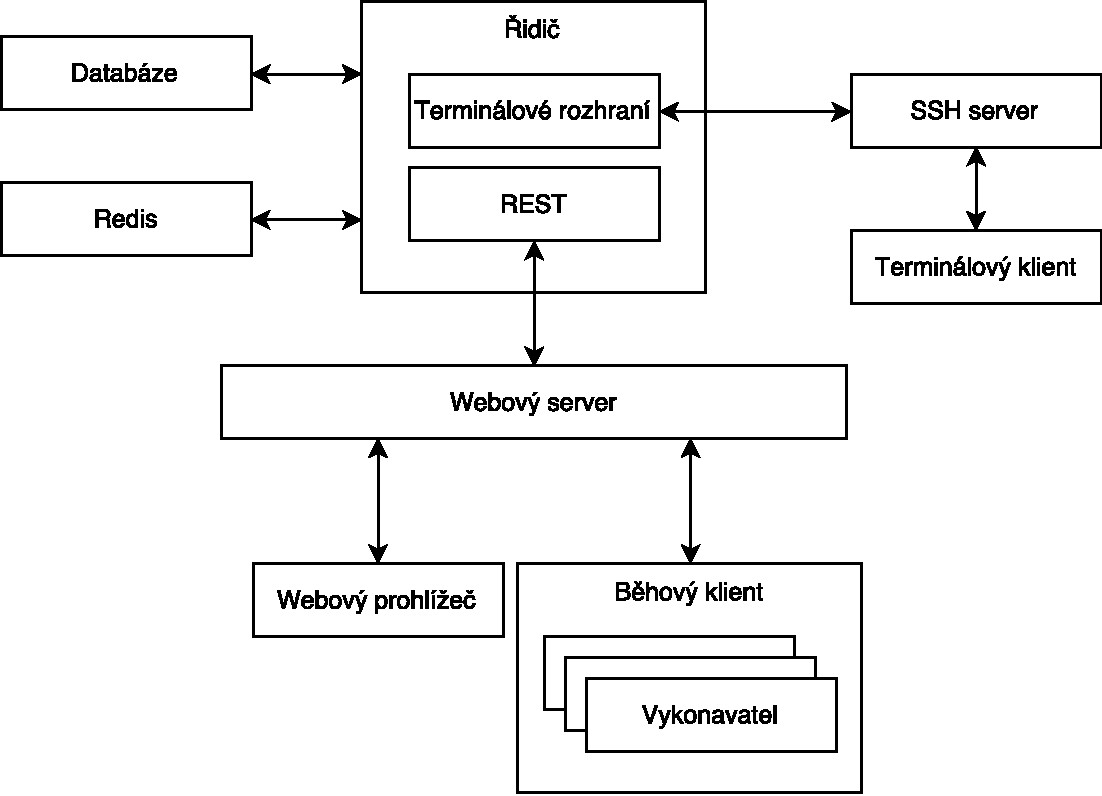
\includegraphics[max width=\linewidth]{architektura_piper.pdf}

\subsection{Řidič}

Zajišťuje komunikaci s~uživatelem, informačním rozhraním a Runnery na pevně daném protokolu.
Řidič by měl být podle vytížení Runnerů (API endpoint na Runneru) a požadovaných služeb rozhodnout, kterému Runneru práci předá.

\subsection{Běhový klient}

Zadaný API vstup rozparsuj pro potřeby Exekutoru a nech ho provést dané příkazy.
Runner by měl spravovat pouze jeden typ exekutoru (Unixová architektura).
Runner by měl běžet na samostatném stroji, aby neubíral systémové prostředky ostatním.
Runner v~sobě většinou bude spouštět více instancí Exekutoru.

\subsubsection{Vykonavatel}

Konečný vykonavatel příkazů. Řidič by neměl o~existenci exekutorů vědět a komunikovat pouze s~Runnery.
Exekutorem je například VirtualBox, Docker a jiné.
Samotná exekutor by měl být co nejméně modifikovaný.
Nechceme například aby VirtualBox exekutor přijímal pouze image, které mají nainstalovaný nějaký obsáhlý set závislostí.

\subsection{Webové rozhraní}

JS only

\subsection{Terminálové rozhraní}

TODO

\input tex/navrh/komunikace
% \input tex/navrh/komunikace_system
% \input tex/navrh/komunikace_system_behove
% \input tex/navrh/persistence_dat
% \input tex/navrh/paralelizace
